\chapter{Сокрытие в спектральной области}
\section{Общие сведения}

\section{Дискретное косинусное преобразование}
Дискретное косинусное преобразование (ДКП) --- одно из дискретных преобразований Фурье.
ДКП представляет конечную последовательность в виде суммы функций косинуса,
колеблющихся на разных частотах. ДКП широко используется при обработке сигналов и сжатии данных.
Например, ДКП используется при сжатии в изображениях (JPEG, HEIF), аудиофайлах (Dolby Digital, MP3),
видеофайлах (MPEG, H.26x), в цифровом телевидении (SDTV, HDTV, VOD) и в других.

ДКП является линейным ортогональным преобразованием. Как любое дискретное линейное преобразование,
ДКП можно представить в виде матрицы. Буду ортоганальным преобразованием, обратное к ДКП преобразование
задает транспонированной матрицей ДКП, домноженной на какой-то коэффициент.

Использование косинусных, а не синусоидальных функций имеет решающее значение для сжатия,
поскольку для аппроксимации типичного сигнала требуется меньше косинусных функций.
ДКП подобно дискретному преобразованию Фурье, но использующее только действительные числа.

Существует 8 стандартных типов ДКП, однако наиболее употребимым является второй тип,
который часто называют просто ДКП (DCT-II).
Формула дискретного косинусного преобразования выглядит так,
как показано в формуле~\ref{eq:simple-dcp}:
\begin{equation} \label{eq:simple-dcp}
    X_k = \sum_{n=0}^{N-1} x_n \cos \left[\frac{\pi}{N} \left(n+\frac{1}{2}\right) k \right] \quad \quad k = 0, \dots, N-1    
\end{equation}
Формула для матрицы преобразования выглядит как формуле~\ref{eq:matrix-dcp}:
\begin{equation} \label{eq:matrix-dcp}
    {DCT}\text{-}2_n= \left[\cos (k(l+\tfrac{1}{2})\tfrac{\pi}{n})\right]_{0\leq k,l<n}    
\end{equation}

Как и в случае быстрого преобразования Фурье, существуют алгоритмы быстрого ДКП преобразования.

DCT-II часто используется для сжатия с потерями благодаря своему свойству уплотнения энерегии:
в типичных случаях большая часть информации, которую содержит сигнал, концентрируется в нескольких
первых коэффициентах разложения.

Существуют так же многомерные ДКП, которые получаются из одномерных путем композиции ДКП по каждому измерению.
Вывод такого преобразования для двумерного случая показан в формуле~\ref{eq:2d-dcp}.
\begin{align}
    X_{k_1,k_2} &= \nonumber
    \sum_{n_1=0}^{N_1-1}
    \left( \sum_{n_2=0}^{N_2-1}
    x_{n_1,n_2} 
    \cos \left[\frac{\pi}{N_2} \left(n_2+\frac{1}{2}\right) k_2 \right]\right)
    \cos \left[\frac{\pi}{N_1} \left(n_1+\frac{1}{2}\right) k_1 \right]\\
    &= \sum_{n_1=0}^{N_1-1}
    \sum_{n_2=0}^{N_2-1}
    x_{n_1,n_2} 
    \cos \left[\frac{\pi}{N_1} \left(n_1+\frac{1}{2}\right) k_1 \right]
    \cos \left[\frac{\pi}{N_2} \left(n_2+\frac{1}{2}\right) k_2 \right] \label{eq:2d-dcp}
\end{align}
Здесь $[x_{n_1,n_2}]$ --- матрица до преобразования, и $[X_{k_1,k_2}]$ --- матрица
после преобразования.
В матричном виде это преобразование может быть представлено так, как показано
в формуле~\ref{eq:2d-matrix-dcp}, где $x$ --- матрица, которую нужно преобразовать.
\begin{equation} \label{eq:2d-matrix-dcp}
    X = ({DCT}\text{-}2_n) x ({DCT}\text{-}2_n ^ T)
\end{equation}
Именно такое преобразование используется при компрессии в JPEG.

\section{JPEG}
JPEG является широко используемым методом сжатия с потерями для цифровых изображений.
Степень сжатия регулируется, что позволяет выбирать между качеством и размером изображения.
JPEG наиболее широко используемый стандарт сжатия изображений в мире и
наиболее используемый формат цифровых изображений.

ДКП лежит в основе сжатия методом JPEG. Как уже говорилось выше,
ДКП был выбран именно благодаря свойству уплотнения энергии. Чтобы прояснить,
о чем идет речь, мной была сделана визуализация преобразования ДКП.

Выберем на изображении область 32x32 пикселя, как показано на рисунке~\ref{img:lenna-eye}.

\begin{figure}[ht!]
    \centering
    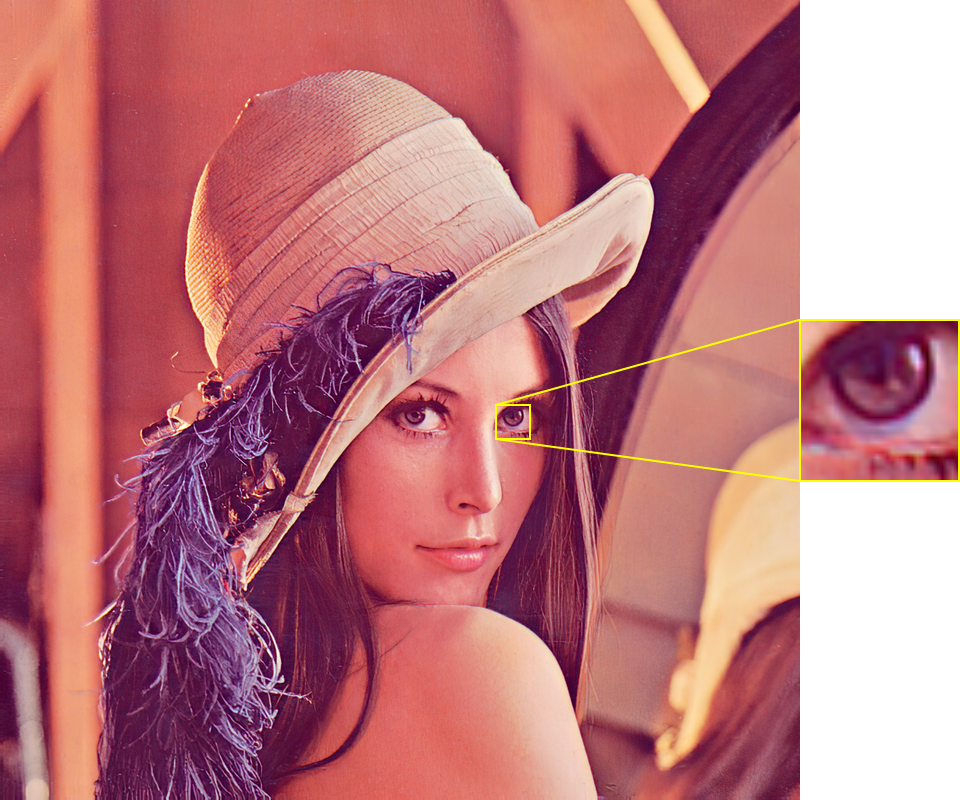
\includegraphics[width=\linewidth]{DCT/Lenna_eye.png}
    \caption{Выбираем область}
    \label{img:lenna-eye}
\end{figure}

%Для простоты будем использовать только синий канал изображения.
Сначала рассмотрим матрицу пикселей как двумерную дискретную функцию.
Расположим координаты так, чтобы в левом верхнем углу
располагался пиксель с координатами $p_{kj}, k = 0, j = 0$.
Визуализацию можно посмотреть на рисунке~\ref{img:pixels-dct}.

\begin{figure}[ht!]
    \centering
    \caption{Визуализация пикселей}
    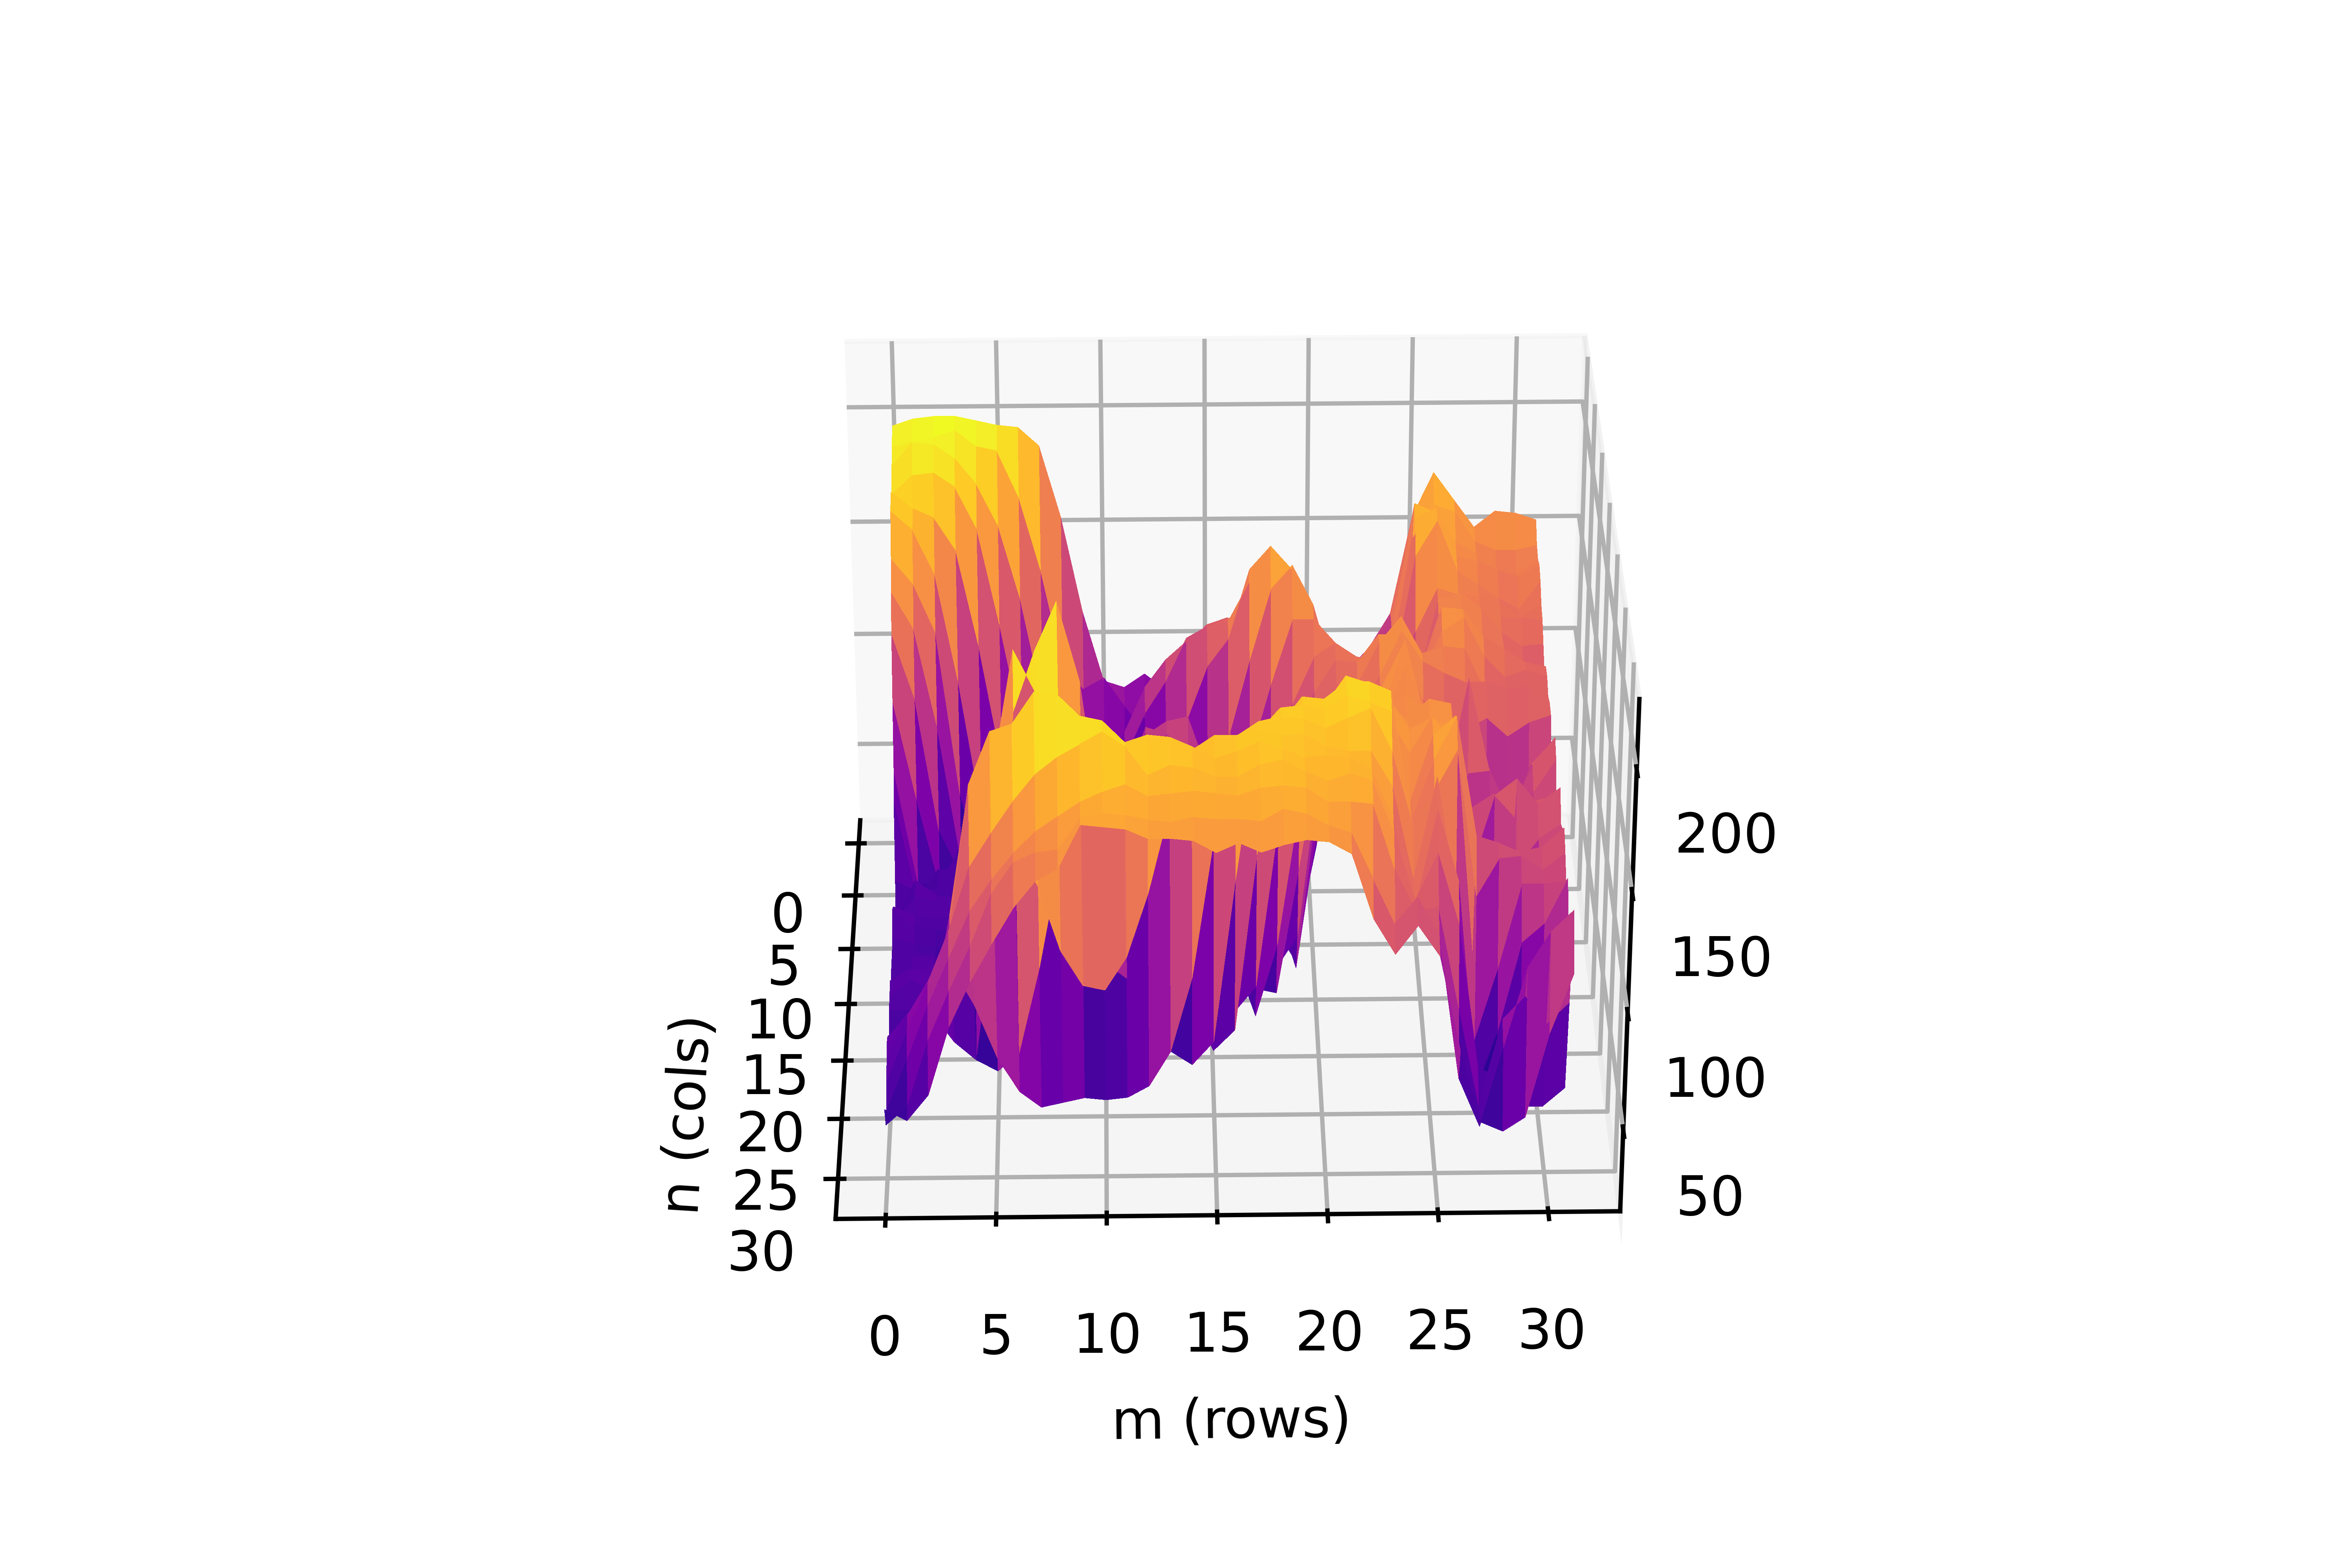
\includegraphics[width=\linewidth]{DCT/pixels.png}
    \label{img:pixels-dct}
\end{figure}

Умножим эту функцию справа на транспонированную матрицу ДКП
по формуле~\ref{eq:2d-matrix-dcp}. Мы получим новую функцию,
которая показана на рисунке~\ref{img:dct-1}.
Таким образом фактически ДКП применилось к каждой строке матрицы.
Из изображения видно, что наибольшие коэффициенты расположены
в нижней части спектра, то есть ближе к нулевому столбцу.

\begin{figure}[ht!]
    \centering
    \caption{После приминения ДКП к строкам матрицы}
    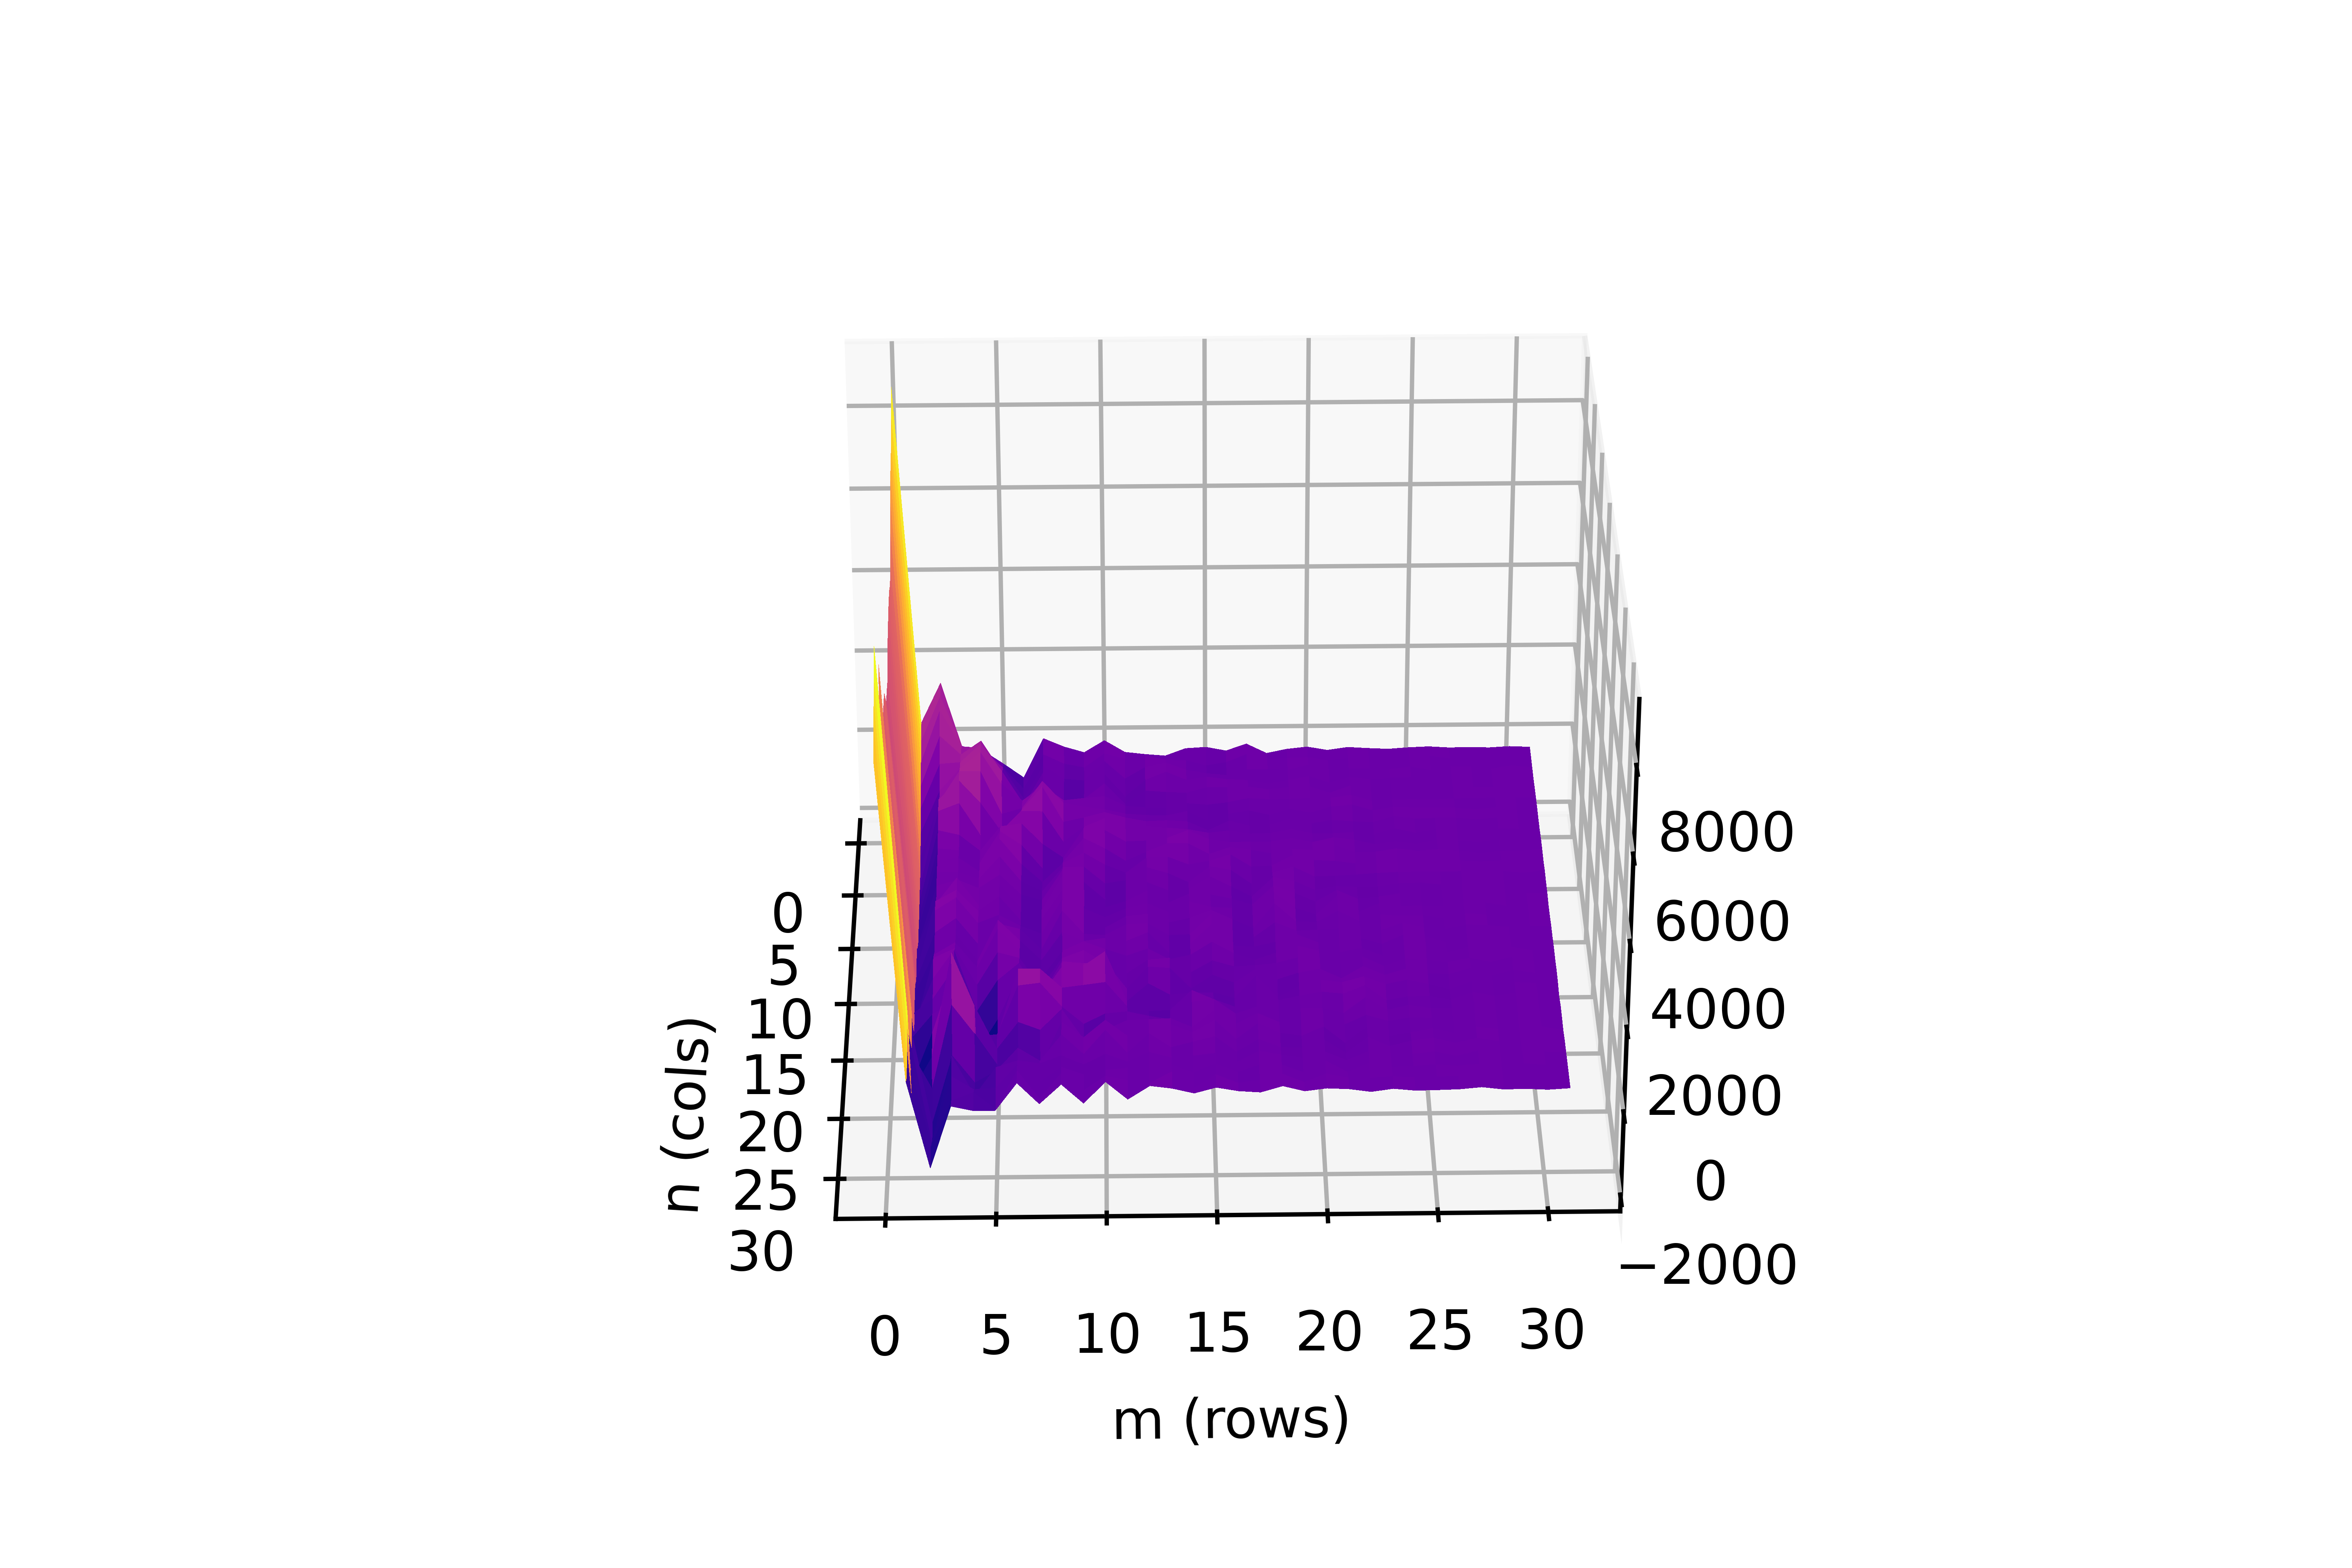
\includegraphics[width=\linewidth]{DCT/dct-1.png}
    \label{img:dct-1}
\end{figure}

К полученной матрице применим ДКП еще раз, в этот раз по столбцам.
В полученной матрице наибольшее значение имеет коэфициент с координатами
$k = 0, j = 0$. Этот коэффициент называется DC-коэффициент.
Остальные коэффициенты называются AC-коэффициентами.
Матрица показана на рисунке~\ref{img:dct-2}.

\begin{figure}[ht!]
    \centering
    \caption{После приминения ДКП к строкам матрицы}
    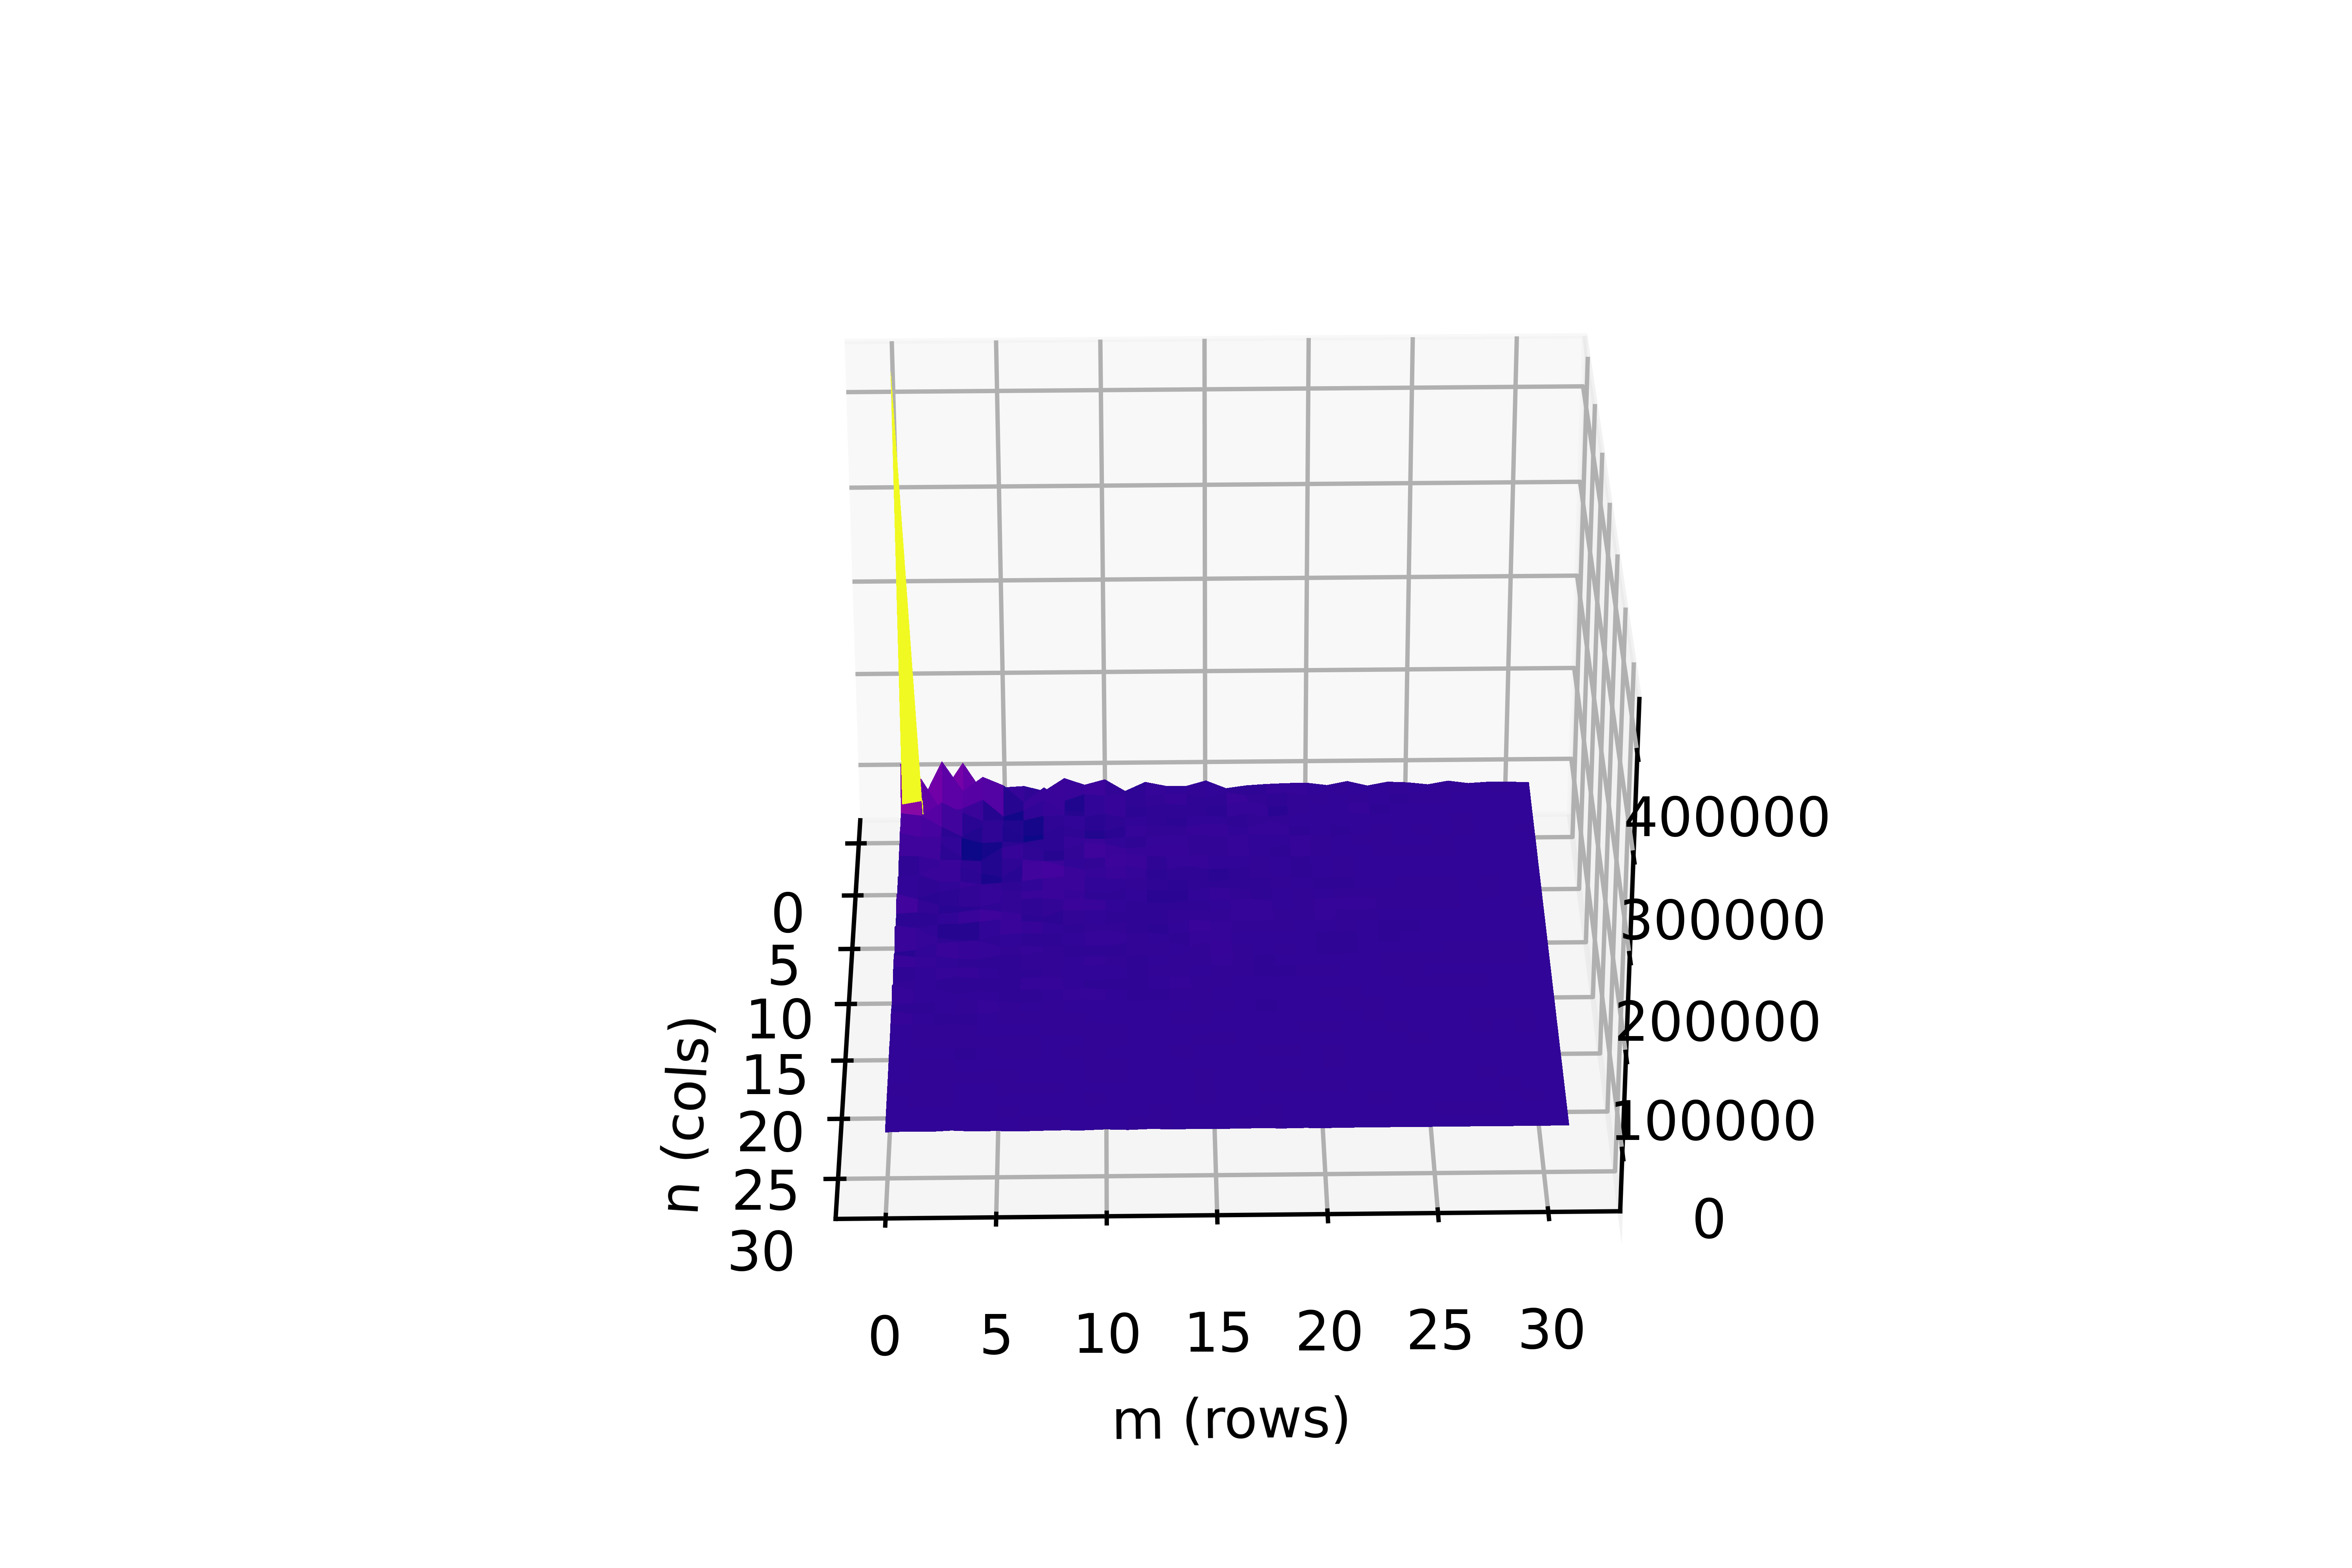
\includegraphics[width=\linewidth]{DCT/dct-2.png}
    \label{img:dct-2}
\end{figure}

DC-коэфициент блока равен среднему всех пикселей в блоке,
взятому с определенным коэффициентом. Удаляя все коэффициенты,
кроме DC, мы можем аппроксимировать блок пикселей их средним
арифметическим. Чем дальше коэффициент располагается от DC,
тем меньше психовизуальной информации он несет для человека,
и тем более незаметные детали изображения он хранит в себе.